\chapter*{Findings}
\begin{table}[htb]
    \renewcommand{\arraystretch}{1.5}
    \begin{tabular*}{\textwidth}{|>{\columncolor{red!15}}p{3cm}|p{17.1cm}|}
    \textbf{Finding} & \textbf{Weak Password for User ''Bluey''}\\
    Risk& High\\
    Category&Access Controls\\
    Impact& An attacker can login as the user ''bluey'' and access \ac{ssh}.\\ 
    Description& After finding out the user names in the last finding the tool hydra was used to try to brute force the passwords of the users. Therefore we used the following script: \newline hydra -l bluey -P rockyou.txt 172.16.0.29 ssh -t 4 -V -I 
	\newline
	The file "rockyou.txt" provided by kali linux includes a list of popular passwords. The hydra script tries to establish a SSH connection by trying every single one of the passwords. With the option ''-t 4'' four passwords are used at once.
	\newline
	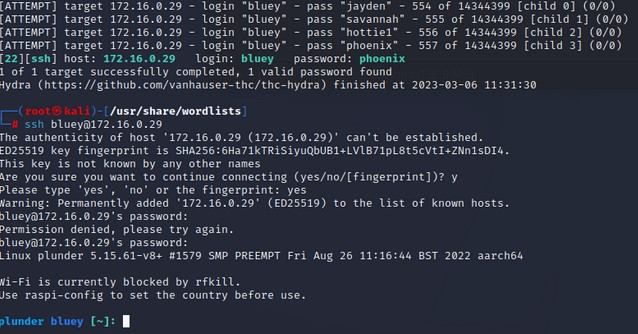
\includegraphics[width = 0.73\textwidth]{brute-force.jpg} 
	\newline
	As shown in the graphic above, Hydra was able to find out the password of the user ''bluey'' which is ''phoenix''. With this information it was possible to establish a SSH connection with the user ''bluey''.
	\\ 
	&\\
    Recommendation& Immediate change password of user ''bluey'' and establish an appropriate password policy.\\    
    \end{tabular*}
    \end{table}